\documentclass[conference,compsoc]{IEEEtran}
\ifCLASSOPTIONcompsoc
  \usepackage[nocompress]{cite}
\else
  \usepackage{cite}
\fi

\ifCLASSINFOpdf
\usepackage[pdftex]{graphicx}
\usepackage{wrapfig}
\graphicspath{ {images/} }
\usepackage[utf8]{inputenc}
  
\else

\fi

\usepackage[cmex10]{amsmath}

\usepackage{lipsum}



\begin{document}

%Probably i can add the name of a specific gesture type from
%a myo pubication 
\title{Gesture to Speech HMI - state of art}

\author{\IEEEauthorblockN{Vladislav Isaak}
\IEEEauthorblockA{Exia Cesi \\Computer Engineering School,\\
Bordeaux, France.\\ 
2017}
\and
\IEEEauthorblockN{Jérôme Brallet}
\IEEEauthorblockA{Exia Cesi \\Computer Engineering School,\\
Bordeaux, France.\\ 
2017}}
\maketitle


\begin{abstract}
Currently, scientists efforts are mostly concentrated on systems that can achieve human parity in conversational speech recognition. By now, the word error rate (WER) of such system is about 5.9 percent that is lower than WER of some professional transcriptionists. A good natural language understanding and its interpretation is mostly achieved by using a variety of powerful Long Short Term Memory Artificial Neural Networks (LSTM NN) \cite{lstm1}. This led to the emergence of many smart assistants for example Cortana, Siri, Alexa and new born but promising Viv. Behind all this there a not less important theme of translation human gestures to natural language. More precisely, hand gestures translation. Most humans do not even realize while they perform their natural gestures with their hand and fingers but some of them do. They do because it's either a part of their work or rehabilitation program, like in case of a ramp marshals or physically injured people, either because it's their only way to communicate like in case of those who suffer from hearing impairment. A breakthrough in this domain might be a significant boost for physical rehabilitation programs in medical institutes, sign language translation applications, training programs requiring a performance of precise gestures and people who are forced to work in an environment not allowing a normal verbal communication. In this paper recent studies in gesture recognition domain combining with Text To Speach (TTS) last achievements \cite{wavenet} will be discussed and analyzed to give you a full understanding of how the state-of-the-art technologies call allow us to build a robust Gesture To Speech (GTS) solution.


\end{abstract}
\textbf{Keywords:} gesture, text to speech, recognition, gesture translation, feature selection, classification, myo armband, emg, imu.

\IEEEpeerreviewmaketitle

\section{Introduction}
Let's start our discussion by defining a scope of this paper. An ordinary human body is flexible enough to perform a hundred or maybe thousands of different gestures with each of its part. Of course, a gesture performed with each part requires a different approach in order to be correctly captured. A system able to capture and to interpret movements of legs, hands and head with the same accuracy should be either overwhelmingly complex either it must have a capacity to modify its own behavior in order to adapt to different use cases.  In this paper, we'll provide a state-of-the-art in GTS only for gestures performed with arms with an amplitude that can be seen effortlessly.

The GTS process itself can be divided into three main parts: Data acquisition, data interpretation and interpretation result transformation into desired form. Each part represents a separate challenge that can be performed separately but in order to obtain a functional system each of three parts must be agreed with others. So, a change in data acquisition process will influence a data interpretation process which in its turn will lead to modifications in results transformation process.  

\begin{figure}[h]
\caption{A high-level overview of GTS process}
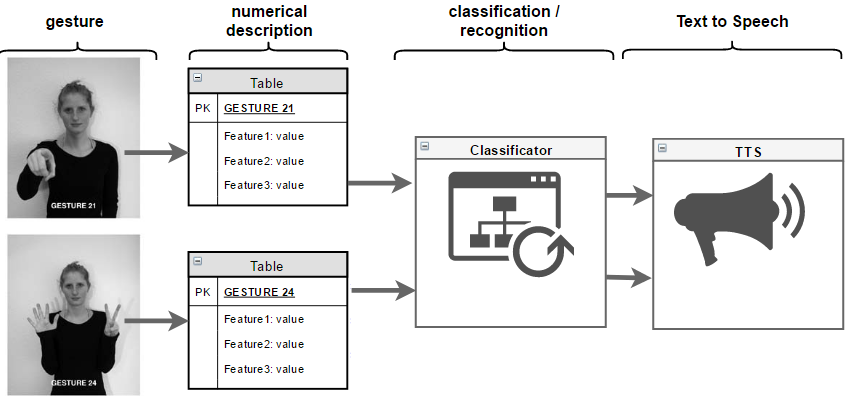
\includegraphics[scale=0.35]{gts_overview}
\centering
\end{figure}

This paper will follow the logic order of GTS process. In the beginning the data acquisition process will be discussed alongside with different methods of data gathering depending on desirable features. Also we'll discuss a feature selection theme. Then we'll see some latest researches in gesture recognition domain. By the end well talk about how we can take advantage of Google Cloud SDK during this kind of research.


\label{tab:examples}

\section{Data Acquisition}
\subsection{Features}
To be able to perform gesture analysis we need to gather data in first. For this it's necessary to find a way to objectively represent gestures using pre-defined parameters. So, what are the features that can be useful in gesture description? Since we are living in three-dimensional world, the first thing that comes into mind is an arm position in the space using X, Y, Z coordinates. But there is a problem in this solution. Spacial  coordinates describes generally a position relative to the origin point. In case if the GTS system will be used by different people in different environments, the origin point will change every time. Static origin point is useful during motion capture \cite{myo_mocap}. But in solution where a person can start using the gesture recognition system in any moment \cite{myo_game} we need to use some other parameters. According to the article from CogInfoCom 2016 \cite{gesture_control_capabilities}, acceleration, orientation, and electromyographical data are appropriate features to describe a gesture. Acceleration can indicate the direction and speed of the arm is moving. Orientation obtained from a gyroscope reflects the degree of the rotation of the arm for each axis. Electromyography is a technique for evaluating the electrical activity generated by a muscle under the electrode.


\subsection{Devices}
There are not many ways to obtain all this data.  While acceleration and orientation data can be obtained from some relatively small sensors that can be placed anywhere, EMG data requires the use of sophisticated electrodes. Use of traditional surface electrodes has advantages because we can place them on muscles that move the hand \cite{time_series_comparison}. But due to the complexity of such system, traditional electrodes are not appropriate for applications meant to be used in everyday life. Further, we'll focus on researches that uses a Myo armband device. 
\begin{wrapfigure}{l}{0.18\textwidth}
    \centering
    \caption{Eight EMG electrodes of Myo armband}
    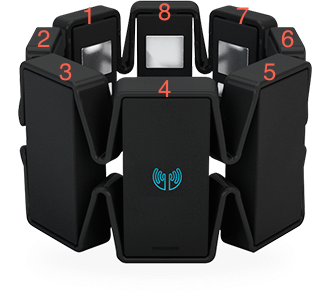
\includegraphics[width=0.17\textwidth]{1zyez3r}
\end{wrapfigure} 
Myo armband developed by Thalmic Lab is more compact and has better appearance compared to traditional electrodes. It has eight electrodes for EMG data and one 9-axis inertial measurement unit (IMU) for spacial data (Orientation, Acceleration, Angular velocity).
But there is an obvious drawback of using Myo. Myo electrodes' are in circular position so we cannot select proper muscles in forearm. Main muscles that covered are Extensor Digitorum and Flexor Digitorum. These are the muscles that move wrist, index, middle, ring, and little finger \cite{time_series_comparison}.

\subsection{Feature selection}
At this point we have a lot of data (17 time-series for each armband), but not all of it is useful. Also, raw sensors data might not be in an appropriate form. Feature selection step will allow us to keep only pertinent data transformed into more informative form.  This is not a trivial task that depends on results we want to obtain and classification method that we’ll be using. Analyzing research paper, I saw that there is no unique method to use armband’s data. However, it may provide some insight on what are features that can be used. In paper from IES 2015 \cite{time_series_comparison} we’ll find a comparison of five ways to represent EMG data (Mean Absolute Value (MAV), Variance (VAR), Willison Amplitude (WAMP), Waveform Length (WL), and Zero Crossing (ZC)). 
\begin{center}
Example of MAV and VAR formulas
\end{center}
\begin{equation}
MAV = \frac{1}{N}\sum_{k=1}^{N}|X_k|
\end{equation}
\begin{equation}
VAR = \frac{1}{N-1}\sum_{k=1}^{N}X_k^2
\end{equation}
This paper recommends the use of MAV value to describe EMG series but tells nothing about IMU data. Prajwal Paudyal\cite{spectre} uses differed approach. He shows that some high-level features (roll, pitch, yaw) can be obtained from IMU data but he does not transform EMG data. He also uses a group sophisticated procedures to combine data from two armbands and normalize it.

\begin{figure}[h]
\caption{Roll, Pitch, Yaw}
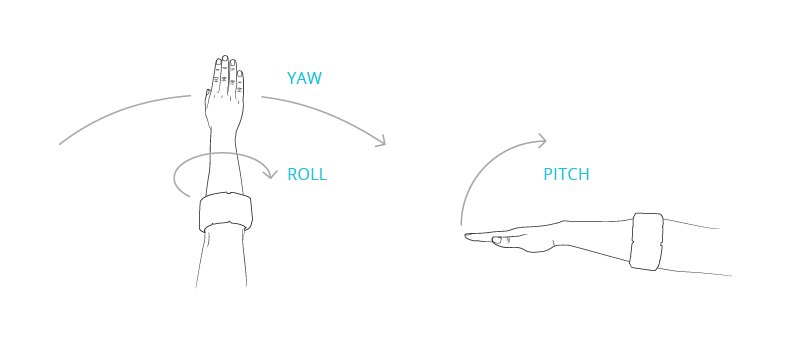
\includegraphics[scale=0.30]{yawetc}
\centering
\end{figure}

\section{Data classification}

The goal of this process is relatively simple. We need to recognize known patterns in provided data. But the actual process is very difficult. Three main questions to ask are: How accurate it should be? How fast it should be? Should it be a real-time solution. The last question is probably most important because it can drastically influence choose of classificator. If the answer is no, user must indicate somehow the beginning and the end of gesture. It can be done by pressing Start-Stop button. The classification process will be simplified but such operational mode will ruin usability. On the other hand, a real-time solution will not bother final users. But such a system must be able to spot known patterns from a constant flow of data. 

During 59th MWSCAS a parer dealing with this problem \cite{algorithm_for_efficient_hci} was presented. It describes how to build a real-time solution using 2D principal component analysis (2DPCA) and canonical correlation analysis (CCA). This paper shows good results in recognition of gestures performed with entire arm but it does not treat gestures performed with fingers. 
Another example of a real-time classificator is described in a publication from 4th GCCE \cite{posture_and_gesture_recognition}.  They used Ordered Subspace Clustering (OSC) and spectral version of Collaborative Representation based Classification (CRC) to create a training dictionary and recognize gestures. But, unlike previously cited paper, here only gestures with fingers are processed. Also, IMU data is not used during model training.

\begin{figure}[h]
\caption{Visualization of 8 EMG signals}
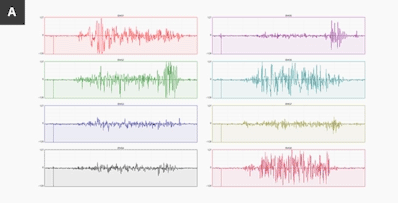
\includegraphics[scale=0.8]{emgsig}
\centering
\end{figure}

These are two main research that worth attention if we want to build a real-time solution. The other papers explore solutions like SVM, SPM, LSTM \cite{sign_language_recognition} and DTW \cite{spectre}. Some of them shows almost 98\% accuracy but they all require a manual indication of where the start and the end of the signal to classify.

Nevertheless, we need to remember that same classifcator can be very powerful or useless depending on features used during its training. 


\section{Results representation}
When the classification process is done and we have obtained desirable results it's time decide what we'll do with them.  This is the last and probably the easiest part of GTS system. There are two main ways to represent data. First, it's possible to represent data as text. Otherwise we can use Text to Speech system that will be able to pronounce the meaning of recognized gestures. Or, a voice command system to control GTS application. For both tasks, we can use Google Cloud SDK that provides multiple services. For example, cloud database can be used to contain mappings from sensors data to words. Google Cloud Machine Learning and Computing platforms can be useful during predicting model training. Also, some of cloud services are able to process real-time data \cite{sign_language_recognition}. 

\section{Conclusion}

Myo armband is a relatively new device and there are no many papers describe how to use it to recognize gestures. Also, it seems that no research was performed to build a system that able recognize both arm gestures and finger gestures on the fly. However, many existing solutions shows a good level of accuracy because of restricted context. In order to create general GTS system, we need either try to combine existing solution either perform further research.

\subsection { GTS in industrial maintenance}
	As we speak about a maintenance in an industrial environment there is unlimited number of applications for a "gesture to speech" system. It can be used as a part of a hand-free interface. It can be useful if a normal communication is not possible due to a noisy environment. A GTS application can translate workers' gesture into speech that will be sent to some other person. Another way to use a GST system is to manipulate machinery from a distance using only gestures. However there is almost no existing GTS solutions applied to industrial maintenance domain. 


\begin{thebibliography}{9}
\bibitem{time_series_comparison} 
Zainal Arief, Indra Adji Sulistijono, Roby Awal Ardiansyah. 
\textit{Comparison of Five Time Series EMG Features Extractions Using Myo Armband}. 
2015 International Electronics Symposium (IES).

\bibitem{gesture_control_capabilities} 
Adam B. Csapo, Árni Kristjánsson, Hunor Nagy, György Wersényi. 
\textit{Evaluation of Human-Myo Gesture Control Capabilities in Continuous Search and Select Operations}. 
7th IEEE International Conference on Cognitive Infocommunications (CogInfoCom 2016) • October 16-18, 2016 • Wrocław, Poland.

\bibitem{posture_and_gesture_recognition} 
Ali Boyali, Naohisa Hashimoto and Osamu Matsumoto. 
\textit{Hand Posture and Gesture Recognition using MYO Armband and Spectral Collaborative Representation based Classification}. 
2015 IEEE 4th Global Conference on Consumer Electronics (GCCE). 

\bibitem{myo_game} 
Karen Yang, David Pan. 
\textit{Myo the Force Be With You}. 
Stanford EE 267, Virtual Reality, Course Report, Instructors: Gordon Wetzstein and Robert Konrad. 

\bibitem{algorithm_for_efficient_hci} 
Ehab H. El-Shazly, Moataz M. Abdelwahab, Atsushi Shimada and Rin-ichiro Taniguchi. 
\textit{Real Time Algorithm for Efficient HCI Employing Features Obtained From MYO Sensor}.
2016 IEEE 59th International Midwest Symposium on Circuits and Systems (MWSCAS), 16-19 October 2016, Abu Dhabi, UAE). 

\bibitem{wavenet} 
Aaron van den Oord, Sander Dieleman, Heiga Zen, Karen Simonyan, Oriol Vinyals, Alex Graves, Nal Kalchbrenner, Andrew Senior, Koray Kavukcuoglu. 
\textit{WAVENET: A GENERATIVE MODEL FOR RAW AUDIO}. 
Google DeepMind, London, UK.

\bibitem{spectre} 
Prajwal Paudyal, Ayan Banerjee, and Sandeep K.S. Gupta. 
\textit{SCEPTRE: a Pervasive, Non-Invasive, and Programmable Gesture Recognition Technology}. 
Arizona State University, Tempe, Arizona). 

\bibitem{sign_language_recognition} 
Hardie Cate, Fahim Dalvi, Zeshan Hussain. 
\textit{Sign Language Recognition using Temporal Classification}. 
December 11, 2015. 

\bibitem{sign_language_recognition} 
R. Langmann. 
\textit{Google Cloud and Analysis of Realtime Process Data}. 
Duesseldorf University of Applied Sciences/Competence Center Automation Duesseldorf (CCAD), Duesseldorf, Germany. 

\bibitem{myo_mocap} 
Yanbin Xu, Chenguang Yang, Peidong Liang, Lijun Zhao and Zhijun Li. 
\textit{Development of a Hybrid Motion Capture Method Using MYO Armband with Application to Teleoperation}. 
Proceedings of 2016 IEEE International Conference on Mechatronics and Automation August 7 - 10, Harbin, China.

\bibitem{lstm1} 
Dong Wu and Mingmin Chi , Member, IEEE. 
\textit{Long Short-Term Memory with Quadratic Connections in Recursive Neural Networks for Representing Compositional Semantics}. 
Proceedings of 2016 IEEE International Conference on Mechatronics and Automation 2016 IEEE.


\end{thebibliography}

\end{document}